%%%%%%%%%%%%%%%%%%%%%%%%%%%%%%%%%%%%%%%%%%%%%%%%%%%%%%%%%%%%%%%%%%%%%%%%%%%%%%%%%
%
% Purpose:  Analysis part of User's Guide for the ModelName model
%
% 
%
%%%%%%%%%%%%%%%%%%%%%%%%%%%%%%%%%%%%%%%%%%%%%%%%%%%%%%%%%%%%%%%%%%%%%%%%%%%%%%%%

% \section{Analysis}
\label{sec:User_Analysis}
\subsection{Overview of the Time Representations}
Typically, a simulation will contain a \textit{time} object, which will
contain a time manager, and possibly some additional number of time
representations.  There are three fundamentally distinct time concepts
working in JEOD:


\begin{itemize}
\item Simulator Time
\item Dynamic Time
\item Derived Time
\end{itemize}



Simulator Time provides the behind-the-scenes simulator control.  For
Trick users, this is the value \textit{sys.exec.out.time.} It provides
the information necessary to ensure that functions are called in the
appropriate order, that tasks are queued appropriately, and to query
whether a task has already been completed.  In general, it must be
incremental, i.e. always advancing forwards.  Simulator Time is not a
part of the \timeDesc, since it does not measure a physical passage of
time.

Dynamic Time is the time used for representing the physics.  When
physical constants rely on a timescale (e.g. speed of light, meters
\textit{per second}), it is the Dynamic Time to which they refer.
Consequently, this is the time used by the integrators.  The Dynamic
Time is automatically included with the Time Manager.

Derived Time has unbounded possibilities, with the ability to represent
any clock that the user chooses, as long as that clock is somehow
related to Dynamic Time.  To find which times are available, open the
S\_define file, find the \textit{time }object, and look for statements
similar to these following:

\begin{verbatim}
 environment/time:  TimeTAI   tai;
 environment/time:  TimeUTC   utc;
 environment/time:  TimeUT1   ut1;
\end{verbatim}

There will be one of these statements for each additional Derived Time.
Within the concept of Derived Time, there are two sub-concepts:


\begin{itemize}
\item Standard Time
\item User-Defined Time
\end{itemize}
These are described in more detail below.

\subsubsection{Dynamic Time (\textit{manager.dyn\_time}, class \textit{TimeDyn})}
The Dynamic Time must be present in any simulation, but will not
appear by itself in the S\_define file.  It always has initial value 0.0, and
counts the number of SI seconds (\textit{manager.dyn\_time.seconds) }elapsed
since the simulation began.  Note that this may not be the same as the
Simulator Time (e.g. \textit{sys.exec.out.time}), since
Dynamic Time has the capacity to run at different rates -- even
in reverse -- whereas the simulator clock is simply an incremental
counter.  The simulation dynamics are all based on Dynamic Time.

\subsubsection[Standard Times (class TimeSTD)]{Standard Times (TimeSTD)}
The concept of a Standard Time is that it is commonly accepted, with no
ambiguity.  Picking a particular value on a particular clock (e.g. noon
on January 23, 2009, UTC) is well understood without additional
context.  Consequently, there can be only one clock running in a
simulation for each of these times (any more would be redundant).
JEOD 2.0 is released with
the following commonly used Standard Times, although this list may have been
extended by your simulation developer.


\begin{itemize}
\item TAI (International Atomic Time) is the most closely linked to
Dynamic Time.  It ticks at the same rate, but starts with a simulation-specific
initial value, defined by the user.  Most derived times are derived
from TAI; this is found in almost all simulations.
\item UTC (Coordinated Universal Time) is the standard clock on Earth.
If initializing the simulation at a particular time, this is usually
handled with UTC.  It ticks at the same rate as TAI, but occasionally
has leap seconds introduced to keep it near-synchronous with UT1.  The
historical record of the occurrence of leap seconds is provided.  If a
simulation happens to span a time at which a leap second was
introduced, UTC will be updated accordingly.  The user may override the
value corresponding to the offset between TAI and UTC, as described in the \reftext{data override section}{ref:data_override}.
\end{itemize}

\begin{itemize}
\item UT1 (Universal Time) is based on the solar day (whereas UTC is
based on days of 86,400 SI seconds).  It ticks at an irregular
rate, a result of a variable rotation rate of Earth, caused by
tidal friction, polar motion, and tectonic action, among others.  The
difference between UTC and UT1 is therefore variable, and not highly
predictable, although it is always less than 1 second (when the
differences become too large, a leap second is added to UTC to bring
them close again -- see figure \ref{fig:TAIUTCUT1}.  For historical simulations, calibrated data is
provided to convert directly from TAI to UT1.  For simulations outside
the range of the provided data, the offset will be held at the last
known value; no attempt is made to predict offsets.  Instructions for
overriding this value are provided in the \reftext{data override section}{ref:data_override}.  Instructions for updating
the calibrated data set with the most recently available data are provided in the \reftext{data update section}{ref:data_update}.


\begin{quotation}
Special Notes Re: previous versions of JEOD:
\begin{enumerate}
\item In this version, the offsets between TAI and UTC, and between
TAI and UT1, are updated continuously, whereas the time management in JEOD 1.x.y identified the offset
at the start of the simulation only, and used that offset throughout
the simulation.  For backward compatibility, the new updates can be
turned off by setting the flags true\_utc and true\_ut1 to
false. This should only
be done for tests that require backward compatibility for comparison to
simulations conducted in JEOD 1.x.
\item In JEOD 1.x.y, the data for generating UT1 was simply the DUT1 value - the difference between UTC and UT1.  In JEOD 2.0, UTC is no longer the ``fundamental'' second, and the preferred conversion method to get UT1 is to do so from TAI.  Therefore, simply using DUT1 to override the tai\_to\_ut1 conversion value will produce error.  The conversion must be from TAI to UT1, therefore attempting to override the data requires additional consideration of the number of leap seconds (UTC to TAI conversion) in order to generate the TAI to UT1 conversion.  Alternatively, a converter could easily be written to generate UT1 from UTC directly, but this has been deliberately omitted from the general release to avoid confusion over identifying the preferred method for generating UT1.  Overriding the data is not recommended for general practice.
\end{enumerate}
\end{quotation}



\begin{figure}[htp]
\begin{center}
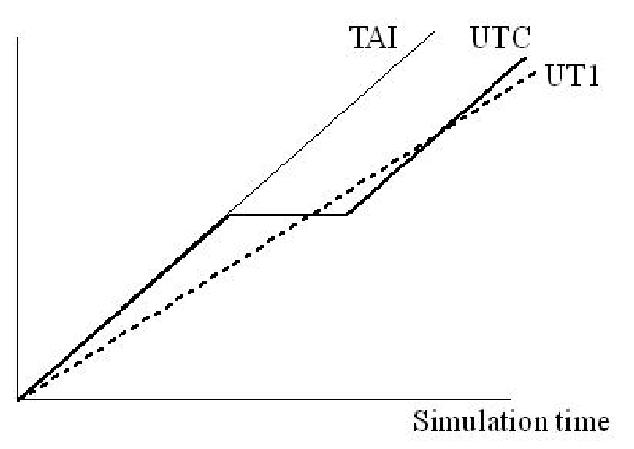
\includegraphics[width=3.2736in,height=2.85in]{figures/Timetaiutcut1.jpg}
\caption{Illustration of the relative evolution of TAI, UTC, and UT1
values, and how leap seconds are used.}
\label{fig:TAIUTCUT1}
\end{center}
\end{figure}


\item GMST (Greenwich Mean Sidereal Time) is based on a sidereal clock
(1 sidereal day = 1 rotation period, approximately 23 hours and 56 minutes
on a synodic clock).  There are 24 sidereal hours in a sidereal day, 60
sidereal minutes in a sidereal hour, and 60 sidereal seconds in a
sidereal minute, although these are rarely -- if ever -- used.
\item GPS (Global Positioning System time) ticks at the same rate as TAI
and is simply offset by a known value, but counts in weeks and seconds
of week rather than days, or the conventional calendar found in TAI.
\item TT (Terrestrial Time) ticks at the same rate as TAI, and is simply
offset by a known value.  It is used in ephemeris models.
\item TDB (Barycentric Dynamic Time) ticks at an obscure rate that
accounts for the relativistic corrections introduced by
Earth's orbital eccentricity.  Since TAI is geocentric
(the clocks are located at the bottom of Earth's
gravitational well, and move with Earth), it is not the best clock for
solar-system missions; TDB removes the geo-effects from TAI.
\end{itemize}



\subsubsection[User-Defined Times (TimeUDE)]{User-Defined Times (TimeUDE)}
The main distinction between a Standard Time and a User-Defined Time is
that User-Defined Times are ambiguous without additional context.  A
commonly used example of a UDE (User Defined Epoch) is Mission Elapsed
Time.  Simply stating that a simulation started two hours after the
mission started is not a very meaningful statement, unless we also have
information on when the mission started.  The \textit{epoch} of UDEs
(i.e. when their value was zero) must be defined before they make any
sense at all; that epoch must ultimately be anchored with a Standard
Time, or with the Dynamic Time.  A secondary difference arises from the
ambiguity of a UDE time; while Standard Times are restricted to one
instance per time-type, the UDEs have no such restriction.  A dozen or
more different clocks could be running simultaneously, representing
different time zones (ticking with UTC), or different mission-elapsed
times for simulations involving multiple vehicles.

There are two types of UDE:


\begin{itemize}
\item UDE:  These have an epoch defined in one time type, and tick in
lockstep with another (may be different).
\item MET (Mission Elapsed Time):  This special type of UDE also has the
ability to halt periodically, to allow for occurrences such as
pre-launch hold points.  The basic UDE will keep ticking through such
hold points.
\end{itemize}



\subsection{Available Data}
This section describes the output data that a user is most likely to
need, identified by the major classes of data.

\subsubsection{JeodBaseTime}
JeodBaseTime is the base class of all time representations.  It contains the
following variables (among others):

\begin{itemize}
\item {\textit{name}} simply names the time object
\item {\textit{days}} represents the current time as some decimal number of elapsed days since epoch
\item {\textit{seconds}} represents the current time as some decimal number of elapsed seconds since epoch
\item {\textit{initial\_value}} is the value of \textit{seconds} at the start of the simulation.
\end{itemize}

\subsubsection[Dynamic Time (time\_dyn)]{Dynamic Time (time\_dyn)}
Dynamic time inherits those data from JeodBaseTime and simply counts SI seconds,
and days, elapsed since the start of the simulation.  It also contains
a variable, \textit{scale\_factor}, that allows it to deviate from the
simulator time (\textit{e.g. sys.exec.out.time}), although changing
this value is not recommended for a beginning user.

\subsubsection[Standard Times]{Standard Times}
The Standard Times also inherit from Time, and add the following
variables:


\begin{itemize}
\item {\itshape
calendar\_year}
\item {\itshape
calendar\_month}
\item {\itshape
calendar\_day}
\item {\itshape
calendar\_hour}
\item {\itshape
calendar\_minute}
\item {\itshape
calendar\_second}
\item {\itshape
trunc\_julian\_time}
\item {\itshape
julian\_date}
\item {\itshape
tjt\_at\_epoch}
\end{itemize}



Truncated Julian Time (\textit{trunc\_julian\_time}) is used as the basic anchor
for each clock, giving each one a basis for measuring ``absolute'' time, and
setting the offsets between the clocks.  It
represents the number of days elapsed since
midnight on May 23 / 24, 1968, as measured in its own clock.
That means that Truncated
Julian Time = 0 in Terrestrial Time (TT) does NOT represent the same
instant as Truncated Julian Time = 0 in Universal Coordinated Time
(UTC).

Julian Date is the original basis for Truncated Julian Time, but has its epoch
much farther in the past, so has fewer available signigificant digits for
precision work.  Like
Truncated Julian Time, it has a distinct value in each clock at any specific
instant in time, and is related to Truncated Julian by:
\begin{equation*}
Julian = Truncated-Julian + 2440000.5
\end{equation*}
in all clocks.
Because of its loss of precision, Julian Date should be used for reference
purposes only.


In most Standard Times (excepting GPS and GMST), \textit{seconds} and
\textit{days} are the primary operational data.  They represent elapsed
time since some fixed epoch (default is J2000, or 12:00 noon TT on January 1,
2000). This is the same instant in time across the different clocks;
the difference between the \textit{trunc\_julian\_time} representation
and the \textit{seconds} representation is best seen in this example:
\begin{quotation}
Terrestrial Time (TT) ticks in lockstep with atomic time (TAI), but they
are offset by a constant value.  The J2000 epoch occurred at the same
instant for both, so \textit{seconds} (since J2000) will be the same
for both since they tick in lockstep.  Conversely, the Truncated Julian
Time {\textquotedblleft}epochs{\textquotedblright} are clock-dependent,
so they occurred at different instants.  Since TT and TAI are offset
from each other, their \textit{trunc\_julian\_time} values will always
differ by a constant amount.
\end{quotation}

The epoch can be easily configured to any desired time, J2000 was chosen simply
because it is a well known data point.
Setting the epoch closer to the simulation
time would give a smaller value on the elapsed time, allowing for more precise
time interval specifications (using J2000 as the epoch does allow microsecond
significance, which is adequate for most purposes).  Note that changing the
epoch WILL NOT affect the precision of absolute time, since that will still be
based on Truncated Julian Time (currently with significance of $O(10^{-5}) s$).
In contrast, the \textit{julian\_date} variable has only millisecond
significance.

To anchor the operational values of \textit{seconds }and \textit{days}
to a fixed time, the value \textit{tjt\_at\_epoch} provides the
Truncated Julian Time at the instant that \textit{seconds = 0.0.}

While seconds and days are trivially incremented throughout the
simulation, the calendar variables require a more time-consuming
update, and so are updated only as necessary.  The simulation developer
may (or may not) have scheduled these, and some time representations
may have calendars that are updated regularly, some rarely, some never.
 To check how often those updates are scheduled, look at the S\_define
file for the statements similar to:


\begin{verbatim}
      {DYNAMICS, environment) environment/time: time.utc.calendar_update(
              In  double  simtime =  sys.exec.out.time);
\end{verbatim}

Note that the simtime argument is used for the purposes of verifying
that the update is actually needed (occasionally, calendar updates are
called behind the scenes by other routines, so if time has not advanced
since it was last updated, it will not be updated again).  The actual
time data is pulled directly from the time object, in this case,
\textit{utc.  }




\subsubsection{User-Defined-Epoch Times (TimeUDE)}
Again, these inherit from Time, but add the following variables:


\begin{itemize}
\item {\itshape
epoch\_year}
\item {\itshape
epoch\_month}
\item {\itshape
epoch\_day}
\item {\itshape
epoch\_hour}
\item {\itshape
epoch\_minute}
\item {\itshape
epoch\_second}
\item {\itshape
clock\_day}
\item {\itshape
clock\_hour}
\item {\itshape
clock\_minute}
\item {\itshape
clock\_second}
\item {\itshape
epoch\_format}
\item {\itshape
initial\_value\_format}
\item {\itshape
epoch\_defined\_in\_name}
\end{itemize}
The \textit{epoch\_***} values are the values of the clock (declared by
name in \textit{epoch\_defined\_in\_name}) at which the UDE time starts
(i.e. has value = 0.0).

The \textit{clock\_*** }values function comparably to the
\textit{calendar\_*** }variables found in the Standard Times; they
provide the dd::hh::mm::ss clock value of the current time, measured in
time elapsed since epoch.  They may also be used to set the epoch of one
UDE by specifying it in terms of the \textit{clock\_***} value of another
UDE.

Note that UDE times do not include year and
month, since these are not well-defined quantities outside of a
standard time reference (a day is 86,400 seconds, while a month is some
variable number of days).

\subsection{Initializing the Simulation}
In any application where specific absolute times are needed (e.g.,
ephemeris), the simulation must be initialized to some known value.  The
start of the simulation always has a Dynamic Time value of 0.0, but may
have a UTC value of 2005/Jan/23::15:30:05 (as an example).
Initialization in this context means setting the starting times
correctly.  This section describes how to do that.




In very basic simulations, there may be no need for an absolute
reference time, nor a second clock.  In that case no additional times
should be declared in the S\_define, and only \textit{dyn-time} used.  Since
\textit{dyn-time} will always start running at 0.0, that eliminates the need for
an initialization process.  The code will terminate if the user
includes any additional clocks (beyond the default Dynamic Time) but
fails to specify a method for initializing the simulation.

Where initialization is required, those values are set in an input file
or modified-data file, discussed below.

\subsubsection{Initialization requirements}
The following is a list of requirements pertinent to initialization.
This is provided as a reference so that the user can identify the
capability of the \timeDesc.


\begin{itemize}
\item The initialization is available from any Standard or UDE time.
\item The initialization time can be expressed in any of the following
formats:

\begin{itemize}
\item Gregorian calendar (Standard Times only)
\item dd::hh::mm::ss clock format (UDE Times only)
\item Julian, Modified Julian, or Truncated Julian formats (Standard Times only)
\item days since epoch
\item seconds since epoch
\end{itemize}
\item Initializing a UDE Time (such as Mission-Elapsed-Time) requires
that the UDE be anchored to another defined time representation.  The
following options are available:

\begin{itemize}
\item Given an absolute UDE epoch time (defined with respect to some
other Derived Time (e.g. 0.0 UDE (tjt)= 123.456 TAI (tjt))) and an
absolute start time from some Derived Time of known epoch (e.g.
sim\_start = 123.456 UTC (tjt)), then the initial value of the UDE time
can be calculated.
\item Given an absolute UDE epoch time and UDE initial value, then the
absolute start time can be calculated and used to initialize other
times, and the simulation.
\item Given an absolute simulation-start time from some Derived Time and
an initial value for the UDE time, then the absolute UDE epoch time
(mission start time) can be determined.
\end{itemize}
\end{itemize}






\subsection{Input Files}
\subsubsection{Defining the initialization time with a Standard Time}
If some real time is to be used to start the simulation, it must be
expressed in some representation (e.g. UTC).  The first value to
specify is that representation, and it must be specified by name.

\begin{verbatim}
time.time_manager_init.initializer ="UTC";
\end{verbatim}




Next, the format in which the time is expressed must be declared.  This
could be Julian, modified\_julian, truncated\_julian, or calendar.
Obviously, the choice is determined by the data available to the user.
The choice must be preceded by
{\textquotedblleft}TimeEnum::{\textquotedblright} as in the example
below.


\begin{verbatim}
time.time_manager_init.sim_start_format = TimeEnum::calendar;
\end{verbatim}

In this case, calendar was chosen, it is now necessary to fully define
the mission start time in a calendar format on a UTC clock.

\begin{verbatim}
time.utc.calendar_year = 1998;
time.utc.calendar_month = 12;
time.utc.calendar_day = 31;
time.utc.calendar_hour = 23;
time.utc.calendar_minute = 59;
time.utc.calendar_second = 50.0;
\end{verbatim}

If the start time were known in a Truncated Julian format on the UT1
clock, for example, this may have looked like:

\begin{verbatim}
time.manager_init.initializer = "UT1";
time.manager_init.sim_start_format = TimeEnum::truncated_julian;
time.ut1.trunc_julian_time = 12345.6789;
\end{verbatim}

The code has some internal verification processes that will catch most
of the common errors that users are likely to make in defining these values,
but it is always
better to get it right the first time.



\subsubsection {Initializing a UDE or MET / Setting the Epoch for a UDE or
MET}

There are two values that all clocks take at simulation-initialization:
\begin{itemize}
\item A definition of its epoch (the time at which it had a value of 0.0)
\item Its value at the start of the simulation.
\end{itemize}

Standard clocks have a default epoch already defined.  Dynamic Time has an
automatic epoch of ``now''.  User-Defined-Epoch clocks (UDE and the more
flexible MET clocks) need additional definition.

Unless the UDE is being used to initialize the simulation, it is necessary
that only one of these is defined.  The other will be calculated.
Specifying both will overconstrain the system and lead to a failure.  If
the UDE is being used to initialize the simualtion, then both must be
specified.

There are multiple ways to directly specify the epoch of a UDE, including:
\begin{itemize}
\item as a calendar date and time in some standard clock,
\item as a Julian, Modified Julian, or Truncated Julian value in some standard
clock,
\item as some number of days or seconds elapsed since, or preceding, the epoch
of another clock (Standard or another UDE)
\item as some number of days or seconds elapsed since, or preceding, the start
of the simulation
\item as some time elapsed since, or preceding, the epoch of another UDE,
expressed in a clock format -- days, hours, minutes and seconds.
\end{itemize}

The sequence for setting the epoch is as follows:
\begin{enumerate}
 \item Decide on the clock to be used to define the epoch.
 \begin{itemize}
  \item Set the variable \textit{epoch\_defined\_in\_name} to the name of the
  chosen clock.  For example,
  \begin{verbatim}
        jeod_time.ude_clock.epoch_defined_in_name = "UTC"
  \end{verbatim}
  \item If setting it relative to simulation-start, use Dynamic Time
  (``Dyn'').
 \end{itemize}

 \item Decide on which option to use to numerically define the epoch.
 \begin{itemize}
  \item Set the value \textit{epoch\_format} accordingly to one of
  \begin{itemize}
   \item \textit{Julian} or \textit{julian}
   \item \textit{modified\_julian}
   \item \textit{truncated\_julian}
   \item \textit{calendar}
   \item \textit{clock}
   \item \textit{days\_since\_epoch}
   \item \textit{seconds\_since\_epoch}
  \end{itemize}
  \item  Note that not all options are available for all clocks.
  \begin{itemize}
   \item If setting relative to Dyn, use only \textit{days\_since\_epoch}
   or \textit{seconds\_since\_epoch}.
   \item If setting relative to another UDE, use only \textit{clock},
   \textit{days\_since\_epoch},
   or \textit{seconds\_since\_epoch}.
   \item If setting relative to a standard clock, use any option other than
   \textit{clock}.
  \end{itemize}
  \item Prepend your selection with \textit{trick.TimeEnum.}.  For example,
  to specify the epoch in a UTC calendar:
  \begin{verbatim}
        jeod_time.ude_clock.epoch_format = trick.TimeEnum.calendar
  \end{verbatim}

 \end{itemize}

 \item Set the numerical value(s) appropriate to your choice.
 \begin{itemize}
  \item If using \textit{calendar}, assign values to \textit{epoch\_year,
  epoch\_month, epoch\_day, epoch\_hour, epoch\_minute,} and
  \textit{epoch\_second}.
  \item If using \textit{clock}, assign values to \textit{clock\_day,
  clock\_hour, clock\_minute,} and \textit{clock\_second}.
  \item If using any of the other options, assign a value to
  \textit{epoch\_initializing\_value}.  This value is a dimensionless
  variable adopting units appropriate to its usage (i.e. days for the
  Julian and days-since-epoch options, and seconds for the
  seconds-since-epoch option).
  \item The \textit{epoch\_***} and \textit{clock\_***} variables can be set
  directly.  For example:
  \begin{verbatim}
       jeod_time.ude_clock.epoch_year = 1998
       jeod_time.ude_clock.epoch_month = 12
       jeod_time.ude_clock.epoch_day = 31
       jeod_time.ude_clock.epoch_hour = 23
       jeod_time.ude_clock.epoch_minute = 59
       jeod_time.ude_clock.epoch_second = 55.0
  \end{verbatim}
  \item The \textit{epoch\_initializing\_value} must be set with a call
  using the format:
  \begin{verbatim}
       jeod_time.ude_clock.set_epoch_initializing_value(0.0,<value>)
  \end{verbatim}
  The first argument must be 0.0, the second argument is the assigned
  value.
 \end{itemize}
\end{enumerate}

Alternatively, the epoch may be inferred by initializing the simulation
with respect to one clock, and setting the corresponding initial value of
the UDE.
The variable \textit{initial\_value\_format} specifies which data
set to look for  in  setting the initial value.  The options are:
  \begin{itemize}
   \item \textit{clock}
   \item \textit{days\_since\_epoch}
   \item \textit{seconds\_since\_epoch}
  \end{itemize}

If using \textit{clock}, assign values to \textit{clock\_day, clock\_hour,
clock\_minute,} and \textit{clock\_second}.  If using either of the other
options, assign a value to \textit{initializing\_value}.
Like \textit{epoch\_initializing\_value}, this value is a dimensionless
variable adopting units appropriate to its usage (i.e. days for the
days-since-epoch option, and seconds for the
seconds-since-epoch option).
The \textit{clock\_***} and \textit{initializing\_value} variables
may be set directly.  For example:
\begin{verbatim}
   jeod_time.ude_clock.initial_value_format = trick.TimeEnum.seconds_since_epoch
   jeod_time.ude_clock.initializing_value = -5.0
\end{verbatim}

This will start the clock with a value of -5.0 seconds, thereby placing its
epoch
5.0 seconds into the simulation.  Equivalently, the epoch could have been
set to be 5.0 seconds after the simulation start-time.  The two examples
presented here -- for setting the epoch and for setting the initial time --
are equivalent when used with the example in the previous section on
initializing the simulation from the UTC calendar representation.

Note that defining initial values for both \textit{initializing\_value} and
any of the \textit{clock\_***} variables will set up an internal conflict
and the code will fail.



\subsubsection{Initializing the simulation with a UDE or MET time}
To initialize the simulation with a UDE or MET time, that time must have
an epoch defined in some other time-type, and have an initial value with
respect to that epoch.  This is best seen in an example, such as at
\textit{verif/SIM\_5\_all\_inclusive/SET\_test/RUN\_UDE\_initialized/input.py}:

\begin{verbatim}
time.manager_init.initializer = "met_veh1"

time.metveh1.epoch_defined_in_name = "UTC"
time.metveh1.epoch_format = TimeEnum::calendar
time.metveh1.epoch_year = 1998
time.metveh1.epoch_month = 12
time.metveh1.epoch_day = 31
time.metveh1.epoch_hour = 23
time.metveh1.epoch_minute = 59
time.metveh1.epoch_second = 0.0

#///////////////////////////////////////////////////////////////////////
#// These two blocks are equivalent
#///////////////////////////////////////////////////////////////////////
time.metveh1.clock_day = 0
time.metveh1.clock_hour = 0
time.metveh1.clock_minute = 0
time.metveh1.clock_second = 50.0
#///////////////////////////////////////////////////////////////////////
#//time.metveh1.initial_value_format = TimeEnum::seconds_since_epoch
#//time.metveh1.initializing_value = 50.0
#///////////////////////////////////////////////////////////////////////

...

time.metveh1.update_from_name = "TAI";
\end{verbatim}
This example will start the \textit{metveh1} clock at a time corresponding to
1998/12/31::23:59:0.0 UTC.
The simulation will start when \textit{metveh1} = 50.0 seconds and
\textit{metveh1} will tick with TAI.
Note -- holds on MET
times can only be processed following simulation start, so in this example,
\textit{metveh1}
must have a value of 50.0 seconds at a time corresponding to 50.0 TAI-seconds
after the epoch time.

Since TAI and UTC are in lock-step during this interval, this example
is equivalent to
initializing the simulation at 1998/12/31::23:59:50.0 UTC, and setting the
initial value of \textit{metveh1} to 50.0 seconds.



\subsubsection{Defining the Trees}
The final part of the input file for time comprises setting up the
initialization and update trees.  Subject to the availability of
converter functions, any time type can (in principle) be initialized or
updated by any other time type.  However, it is recommended that TAI be
derived from Dynamic Time, and other types from TAI; in particular, due to
the implementation of leap seconds, TAI is not uniquely identified from all
UTC values, and TAI should never be updated from UTC.

\begin{verbatim}
time.time_tai.initialize_from_name ="UTC"
time.time_tai.update_from_name = "Dyn"
\end{verbatim}

This states that the initial value of TAI is going to be set by
the initial value of UTC (so there had better be a
UTC to TAI converter available and declared in the S\_define).  Folowing commencement of the simulation, TAI will continue to get its
values based on the value of Dynamic Time (\textit{manager.dyn\_time}). If
the user omits any part of the tree specification, the code has
sufficient capability that it can search for the most direct path to
provide a means of initializing or updating a time type that has no
specified path.  If such a path is found, a low-priority message will
be sent to the message handler to alert the user to the paths selected.
 The code will terminate immediately if any of the following conditions
are met:


\begin{itemize}
\item The user did not specify a full tree, and the auto-generator could
not find a suitable path.
\item The user sets up these paths in such a way that they generate
circular dependency (e.g. type XXX updates from YYY, and YYY from XXX).
\item A path is specified but there is no converter to handle the
conversion.
\item The specified initialization path does not form a continuous
connection from the initializer to each of the time types.
\item The specified update path does not form a continuous connection
from Dynamic Time to each of the time types.
\item The \textit{initializer} has a defined value for its
\textit{initialize\_from\_name} variable
(the \textit{initializer} gets its
initial data from user-input, not from another clock)
\footnote{If editing an existing simulation to use a different clock as the
\textit{initializer}, overwrite the new \textit{initializer}'s
\textit{initialize\_from\_name} so that it is empty (``''), and define a
value for \textit{initialize\_from\_name} for the old \textit{initializer}.}.
\end{itemize}

\subsubsection{Commanding changes mid-simulation}
The \textit{manager.update} routine checks the current Simulator Time with its recording of the Simulator Time the last time the Time Manager was called.
The user may specify changes to various values (e.g., start and stop a MET, change the scale-factor on the Dynamic Time) based on particular events, or on a predetermined Simulator Time-based schedule.  While those changes are implemented before the call is made to the \textit{manager.update} routine for a given Simulator Time, this is insufficient to ensure that the \textit{manager.update} routine is run with those changes set.

The problem lies in the behind-the-scenes interaction between the dynamic integrator and the Time Manager.  With some integrators (e.g. Runge-Kutta 4), the time must be evaluated at the end of the previous step as a component of the previous integration.  So at step \textit{i}, the value for time is needed at \textit{i, i+0.5,} and \textit{i+1}.  Once step \textit{i} is complete, changes made for step \textit{i+1} are implemented, and step \textit{i+1} begins; however, time has already been calculated at \textit{i+1}, and the update will not be called again for this instant of time without further intervention.

Therefore, it is recommended that whenever changes are being commanded, that the Time Manager's recorded value of Simulator Time be manipulated to ensure that when the \textit{manager.update} routine is called, the current Simulator Time will not agree with the recorded value.  A safe value is 0, since Simulator Time starts at 0 and always increments.

\begin{verbatim}
 read = 10
 time.metveh2.hold = true
 time.manager.simtime = 0
\end{verbatim}

\subsubsection{Turning off Warnings}
When setting the time, it is easy to overlook a critical step and finish with an
unrealistic time.  Fortunately, the most obvious errors are easily caught at
initialization by testing the value of Truncated Julian Time.  If it has a value
of
zero or less, a warning will be sent to the Message Handler.  Developers of
those historical simulations for which Truncated Julian Time should be less than
zero (i.e. pre-May 24, 1968) have an option to disable this warning message by
setting the flag \textit{send\_warning\_pre\_1968 = false}.
